\documentclass[conference]{IEEEtran}
\usepackage{amsmath,amssymb}
\usepackage{booktabs}
\usepackage{array}
\usepackage{multirow}
\usepackage{xcolor}
\usepackage{tikz}
\usetikzlibrary{arrows.meta,positioning,calc,fit,backgrounds}
\usepackage{pgfplots}
\pgfplotsset{compat=1.18}
\usepackage{newtxtext,newtxmath}
\usepackage{url}
\usepackage{microtype}
\usepackage{enumitem}
\usepackage{float}
\usepackage{needspace}
\setlist[itemize]{leftmargin=*,nosep}

\definecolor{cblue}{HTML}{2D6F9F}
\definecolor{corange}{HTML}{D97728}
\definecolor{cgreen}{HTML}{2E7D62}
\definecolor{cred}{HTML}{A33A32}
\definecolor{cgray}{HTML}{68737D}
\definecolor{clight}{HTML}{EEF2F4}
\definecolor{clightblue}{HTML}{E6F0F6}
\definecolor{clightgreen}{HTML}{E8F3EE}
\definecolor{clightred}{HTML}{F7E9E7}
\definecolor{clightorange}{HTML}{F8EFE5}

\newcommand{\copycat}{\textsc{CopyCAT}}
\newcommand{\rootcopy}{\mathcal{S}}
\newcommand{\tight}{\vspace{-0.7ex}}

\title{\copycat: Visual Certificate Atlas and Reproducibility Supplement}
\author{\IEEEauthorblockN{Sushanth Dasari}
\IEEEauthorblockA{Amity International School, Sector-46, Gurugram, India\\
Supplementary material for the CopyCAT research manuscript}}

\begin{document}
\maketitle

\begin{abstract}
This supplement is a visual, certificate-first companion to the main \copycat{} manuscript. It deliberately follows a simple progression: first show the phenomenon with no abstraction, then derive the exact pairwise certificate, then explain why one leaderboard winner requires a \emph{shared} schedule rather than separate pairwise witnesses, and finally connect every headline claim to an executable check in the public repository. No new scientific claim is introduced here. The purpose is to make the existing finite-archive result easier to audit: on the pinned 588-question MMLU-ProX-Lite archive, GPT needs exactly three shared copies to become uniquely first, Claude needs exactly eight, and seven other configurations are provably excluded under the one-extra-copy-per-root intervention. The same audit distinguishes targeted attainability from random frequency and motivates a mass-preserving repair once trusted root lineage is given.
\end{abstract}

\section{Start With the Smallest Possible Story}
A benchmark score is an average over units that are intended to count once. \copycat{} asks a deliberately narrow question: if the predictions and labels are frozen, but some \emph{existing} units are allowed to count twice, which decisions can change? The same copied-root set must be used for every system. Nothing about the models changes; only what the evaluator counts changes.

\begin{figure}[H]
\centering
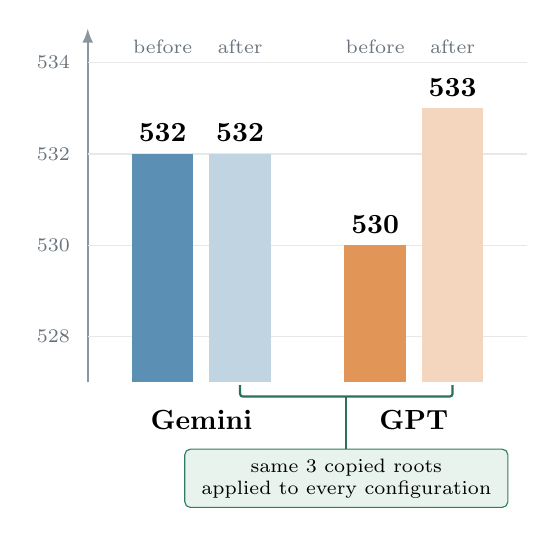
\begin{tikzpicture}[x=0.78cm,y=0.58cm,font=\footnotesize,>=Latex]
  \draw[-{Latex[length=1.8mm]},cgray!75,line width=0.55pt] (0,0) -- (0,7.75);
  \foreach \y/\lab in {1/528,3/530,5/532,7/534}{
    \draw[gray!18,line width=0.45pt] (0,\y) -- (7.15,\y);
    \node[anchor=east,text=cgray,font=\scriptsize] at (-0.13,\y) {\lab};
  }
  \fill[cblue!78]   (0.72,0) rectangle (1.72,5.00);
  \fill[cblue!30]   (1.98,0) rectangle (2.98,5.00);
  \fill[corange!78] (4.18,0) rectangle (5.18,3.00);
  \fill[corange!30] (5.44,0) rectangle (6.44,6.00);
  \node[anchor=south,font=\bfseries] at (1.22,5.05) {532};
  \node[anchor=south,font=\bfseries] at (2.48,5.05) {532};
  \node[anchor=south,font=\bfseries] at (4.68,3.05) {530};
  \node[anchor=south,font=\bfseries] at (5.94,6.05) {533};
  \node[text=cgray,font=\scriptsize] at (1.22,7.35) {before};
  \node[text=cgray,font=\scriptsize] at (2.48,7.35) {after};
  \node[text=cgray,font=\scriptsize] at (4.68,7.35) {before};
  \node[text=cgray,font=\scriptsize] at (5.94,7.35) {after};
  \node[font=\bfseries] at (1.85,-0.82) {Gemini};
  \node[font=\bfseries] at (5.31,-0.82) {GPT};

  % shared-schedule bracket with deliberate breathing room below labels
  \draw[cgreen!90!black,line width=0.8pt,rounded corners=1pt]
        (2.48,-0.06) -- (2.48,-0.31) -- (5.94,-0.31) -- (5.94,-0.06);
  \coordinate (railmid) at (4.21,-0.31);
  \node[draw=cgreen,fill=clightgreen,rounded corners=2pt,align=center,
        inner xsep=6pt,inner ysep=3.4pt,font=\scriptsize] (shared) at (4.21,-2.10)
        {same 3 copied roots\\applied to every configuration};
  \draw[cgreen!90!black,line width=0.8pt] (railmid) -- ++(0,-0.38) -- (shared.north);
\end{tikzpicture}
\caption{The whole headline result before any notation. The outputs and labels are unchanged. Three already-scored roots are counted twice under one common schedule, moving GPT from 530 to 533 correct while Gemini remains at 532.}
\label{fig:headline}
\end{figure}

The lower bound is already visible in Fig.~\ref{fig:headline}. GPT begins two correct answers behind Gemini. A single copied binary root can improve the GPT-minus-Gemini count gap by at most one. A strict win therefore needs at least three favorable copies. The artifact supplies three such roots, so the lower bound is attained.

\section{Now Generalize the Toy Argument}
For a pair of systems $A,B$, let $d_i=z_i^A-z_i^B$ be the fixed score difference on root $i$ and let $D=\sum_i d_i$. If $S$ is the set of copied roots, the new margin is
\begin{equation}
M_{A,B}(S)=\frac{D+\sum_{i\in S}d_i}{n+|S|}.
\label{eq:margin}
\end{equation}
There is no combinatorial mystery in the pairwise case. At exactly $k$ copies, the smallest margin is obtained by copying the $k$ smallest $d_i$ values and the largest margin by copying the $k$ largest values:
\begin{equation}
L_k=\frac{D+\sum_{r=1}^{k}d_{(r)}}{n+k},\qquad
U_k=\frac{D+\sum_{r=n-k+1}^{n}d_{(r)}}{n+k}.
\label{eq:extrema}
\end{equation}
Sorting once therefore gives every exact pairwise budget in $O(n\log n+B)$ time. This sorting principle is established prior work; \copycat{} uses it as one component of a larger shared-schedule audit \cite{alzhrani}.

\begin{figure}[H]
\centering
\begin{tikzpicture}[font=\footnotesize,>=Latex]
  \node[font=\bfseries] at (0,0) {A toy margin certificate};
  \node[text=cgray,font=\scriptsize] at (0,-0.43)
        {baseline count gap $D=-2$; favorable roots have $d_i=+1$};
  \foreach \x/\v in {-3/0,-2/0,-1/1,0/1,1/1,2/-1,3/0}{
    \node[draw=gray!45,fill=white,minimum width=0.57cm,minimum height=0.46cm,
          inner sep=0pt] (r\x) at (0.70*\x,-1.25) {$\v$};
  }
